\documentclass[12pt]{article}

\usepackage{amsmath}
\usepackage{graphicx}
\usepackage{hyperref}
\usepackage{geometry}
\usepackage{tabularx}
\usepackage{array}
\geometry{margin=1in}
\usepackage{float}
\usepackage{amssymb}

\setlength{\marginparwidth}{2cm}
\usepackage{todonotes}

\title{Spacecraft ADCS Homework 2 Report\\
NASA Starling Mission Analysis}
\author{Aleksander Garbuz \\ Israel Garcia}
\date{\today}

\begin{document}
\maketitle

% ==============================
% Changelog
% ==============================

\section*{Changelog}

\begin{center}
\begin{tabular}{| m{3cm} | m{4cm} | m{6cm} |}
\hline
\textbf{Date} & \textbf{Section Modified} & \textbf{Description of Changes} \\
\hline
2026-02-25 & HW1 & Initial report completed \\
2026-03-13 & HW2 & Report 2 \\
\hline
\end{tabular}
\end{center}
\todo{Better changelog}

\todo{Add github link again}
\vspace{1cm}
\section{Safe Mode Spin Design}

\subsection{Safe-Mode Objective}
For a rigid body with three distinct principal moments of inertia, torque-free rotation is stable only about the axes corresponding to the largest and smallest principal inertias; rotation about the intermediate axis is unstable. A dual-spin or gyrostat configuration avoids this limitation by adding internal rotor momentum so that the effective inertia about the desired spin axis exceeds the transverse inertias.

For the Starling-based 6U CubeSat introduced in Section~\ref{sec:model}, the
deployed solar arrays are mounted on the $\pm \mathbf{b}_1$ faces, so the solar
panel normal is aligned with the body $\mathbf{b}_1$ axis. In the body-axis ordering
used previously, this corresponds to the positive body $y$-direction. The objective
of the safe-mode design is therefore to maintain a stable spin about the panel-normal
direction so that the panels remain approximately pointed toward the Sun.

\subsection{Perturbed Inertia Model}

The nominal inertia matrix from the CAD-based HW1 model is aligned with the
spacecraft geometry, which makes the solar panel normal close to a principal
direction. To avoid an artificial special case in which the desired spin axis is exactly
aligned with a principal axis, the inertia matrix was randomly perturbed following the
prescription in the assignment. Let the nominal inertia be decomposed as
\[
\mathbf{I} = \mathbf{V}\mathbf{D}\mathbf{V}^T.
\]
The principal moments were then perturbed according to
\[
\widetilde{\mathbf{D}}
=
\mathbf{D}\left(\mathbf{I}_3 + \mathrm{diag}(\mathbf{d})\right),
\qquad
\mathbf{d} \sim \mathcal{N}\!\left(\mathbf{0}, \sigma_{\mathrm{eig}}^2 \mathbf{I}_3\right),
\]
with $\sigma_{\mathrm{eig}} = 0.03$. The principal-axis directions were perturbed by a
small random rotation,
\[
\widetilde{\mathbf{V}}
=
\mathbf{V}\exp(\widehat{\mathbf{v}}),
\qquad
\mathbf{v} \sim \mathcal{N}\!\left(\mathbf{0}, \sigma_{\mathrm{rot}}^2 \mathbf{I}_3\right),
\]
where $\sigma_{\mathrm{rot}} = 2^\circ$. The perturbed inertia matrix was then reconstructed as
\[
\widetilde{\mathbf{I}}
=
\widetilde{\mathbf{V}}\widetilde{\mathbf{D}}\widetilde{\mathbf{V}}^T.
\]
This perturbation ensures that the solar panel normal is not exactly a principal
direction while preserving a physically realistic inertia tensor.

\subsection{Rotor Momentum Sizing}

The desired safe-mode spin rate was selected as
\[
\omega_{\mathrm{des}} = 10 \ \mathrm{RPM}
= \frac{10(2\pi)}{60}
\approx 1.047 \ \mathrm{rad/s},
\]
about the unit vector $\mathbf{e}$ aligned with the solar panel normal. Because this
axis is not, in general, a principal axis of $\widetilde{\mathbf{I}}$, passive stability is
obtained by adding internal rotor momentum along the same direction.

Let the nominal inertia about the desired spin axis be
\[
J_{s,0} = \mathbf{e}^T \widetilde{\mathbf{I}} \mathbf{e},
\]
and let $J_1$ and $J_2$ denote the inertias about two orthonormal directions
transverse to $\mathbf{e}$. Defining
\[
J_t = \max(J_1, J_2),
\]
the design requirement was chosen to satisfy an inertia ratio of at least
\[
\frac{J_{s,\mathrm{eff}}}{J_t} \geq 1.2,
\]
where $J_{s,\mathrm{eff}} = J_{s,0} + I_r$ includes the added rotor contribution. The
required rotor inertia is therefore
\[
I_r = \max\left(0,\ 1.2\,J_t - J_{s,0}\right),
\]
and the corresponding rotor angular momentum is
\[
H_r = I_r \, \omega_{\mathrm{des}}.
\]

For the perturbed Starling inertia used in the simulation, this calculation yielded
\[
H_r \approx 0.103 \ \mathrm{N\,m\,s},
\qquad
I_r \approx 0.099 \ \mathrm{kg\,m^2}.
\]
These values indicate that only a modest amount of stored rotor momentum is required
to create a gyroscopically stiff safe-mode spin about the panel normal.

\subsection{Gyrostat Attitude Simulation}

To verify stability, the rigid-body attitude dynamics were simulated using the
torque-free gyrostat equations. The body angular velocity $\boldsymbol{\omega}$ and
attitude quaternion $\mathbf{q}$ evolve according to
\[
\dot{\mathbf{q}}
=
\frac{1}{2}\,\Omega(\boldsymbol{\omega})\,\mathbf{q},
\]
and
\[
\widetilde{\mathbf{I}}\,\dot{\boldsymbol{\omega}}
=
-\boldsymbol{\omega}\times
\left(
\widetilde{\mathbf{I}}\boldsymbol{\omega} + \mathbf{h}_r
\right),
\qquad
\mathbf{h}_r = H_r \mathbf{e}.
\]
The initial angular velocity was chosen as the nominal 10 RPM spin plus a 1\%
transverse perturbation in order to demonstrate robustness of the configuration.
The quaternion was initialized as the identity rotation for this standalone
attitude-only test.

Figure~\ref{fig:safe_mode_spin} shows the simulated angular velocity components.
The dominant spin component remains close to the commanded value, while the
transverse components remain bounded and oscillatory. This is the expected response
for a passively stable gyrostat: small perturbations lead to nutation, but not to
runaway growth associated with intermediate-axis instability.

\begin{figure}[H]
    \centering
    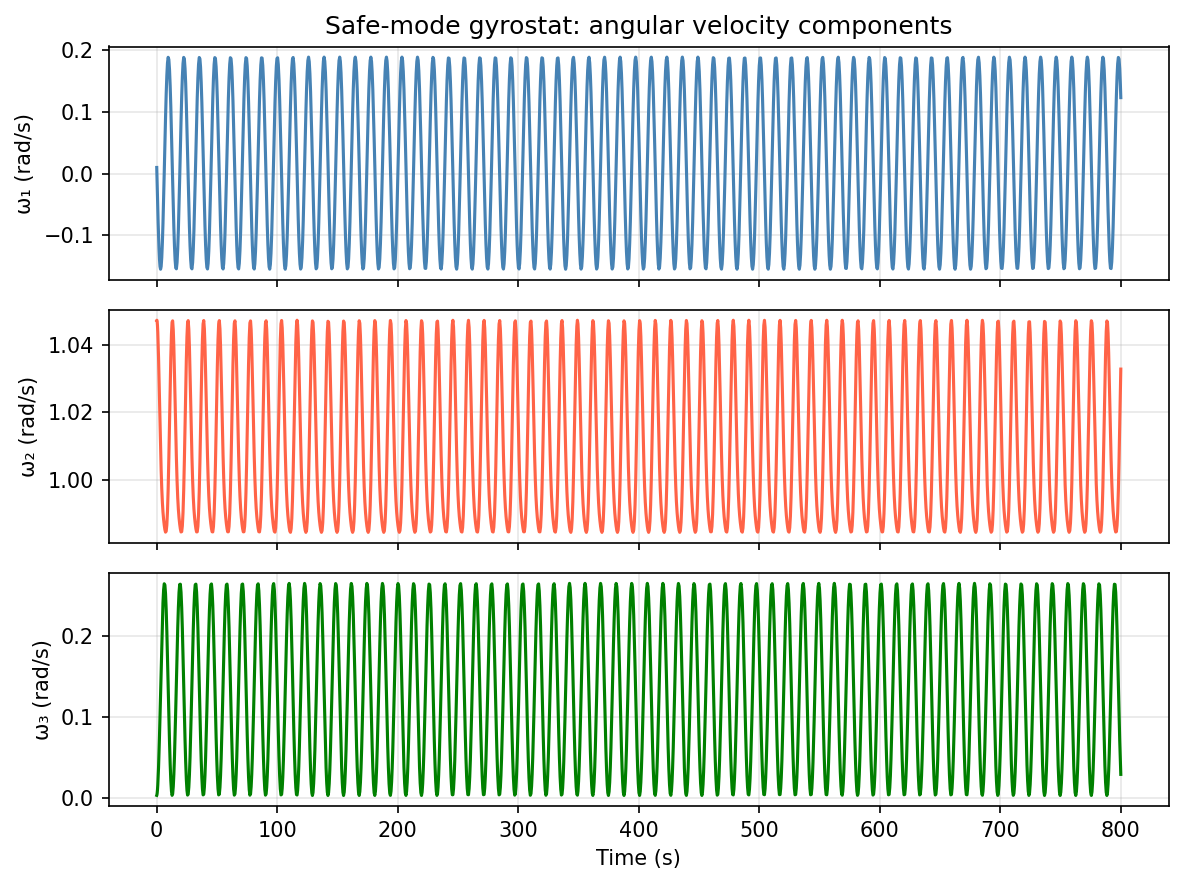
\includegraphics[width=0.78\linewidth]{figs/safe_mode_angular_velocity.png}
    \caption{Safe-mode gyrostat simulation showing bounded angular velocity components under a 1\% perturbation of the initial spin state.}
    \label{fig:safe_mode_spin}
\end{figure}

\section{Spacecraft Dynamics with Gyrostat}

\subsection{Coupled Orbit-Attitude Model}

The second part of the assignment required extending the HW1 orbital simulation to
include gyrostat attitude dynamics. The full state vector was taken as
\[
\mathbf{x}
=
\begin{bmatrix}
\mathbf{r} \\
\mathbf{v} \\
\mathbf{q} \\
\boldsymbol{\omega}
\end{bmatrix}
\in \mathbb{R}^{13},
\]
where $\mathbf{r}$ and $\mathbf{v}$ are the spacecraft position and velocity in the
Earth-centered inertial (ECI) frame, $\mathbf{q}$ is the attitude quaternion mapping
body coordinates to inertial coordinates, and $\boldsymbol{\omega}$ is the body-frame
angular velocity.

The translational dynamics were taken directly from the HW1 model, including
two-body gravity and the $J_2$ perturbation:
\[
\ddot{\mathbf{r}}
=
-\frac{\mu}{r^3}\mathbf{r}
+
\mathbf{a}_{J_2},
\]
where
\[
\mathbf{a}_{J_2}
=
\frac{3J_2\mu R_E^2}{2r^5}
\begin{bmatrix}
x\left(5z^2/r^2 - 1\right) \\
y\left(5z^2/r^2 - 1\right) \\
z\left(5z^2/r^2 - 3\right)
\end{bmatrix}.
\]
Atmospheric drag was omitted for this simulation so that the effect of the coupled
gyrostat dynamics could be isolated.

The rotational dynamics were again modeled with the gyrostat equation
\[
\widetilde{\mathbf{I}}\,\dot{\boldsymbol{\omega}}
=
-\boldsymbol{\omega}\times
\left(
\widetilde{\mathbf{I}}\boldsymbol{\omega} + \mathbf{h}_r
\right),
\]
together with the quaternion kinematics
\[
\dot{\mathbf{q}}
=
\frac{1}{2}\,\Omega(\boldsymbol{\omega})\,\mathbf{q}.
\]

\subsection{Initial Conditions}

The orbit was initialized as the same 480 km circular Sun-synchronous orbit used in
HW1. The inclination was computed from the nodal precession requirement for a
Sun-synchronous orbit, while the remaining orbital elements were selected so that
the ascending node lay along the inertial $x$-axis. The Sun vector was assumed to
be fixed along the inertial $+x$ direction, as specified in the homework statement.

The initial attitude quaternion was selected so that the body-fixed solar panel
normal aligned with the inertial Sun vector at the start of the simulation. The
initial angular velocity was again chosen as the nominal safe-mode spin plus a 1\%
transverse perturbation. This setup is consistent with a spacecraft that has already
entered safe mode and is allowed to evolve freely under its passive gyrostat
dynamics.

\subsection{Simulation Results}

The coupled orbit-attitude equations were integrated for 2000 s, corresponding to
several nutation periods. To evaluate Sun-pointing performance, the instantaneous
pointing error was defined as the angle between the inertial Sun vector
$\mathbf{s}$ and the inertial image of the body-fixed panel normal,
\[
\theta_{\mathrm{err}}
=
\cos^{-1}
\left(
\frac{\left(\mathbf{R}_{BI}\mathbf{e}_{\mathrm{panel}}\right)\cdot\mathbf{s}}
{\|\mathbf{R}_{BI}\mathbf{e}_{\mathrm{panel}}\|\,\|\mathbf{s}\|}
\right),
\]
where $\mathbf{R}_{BI}$ is the body-to-inertial direction cosine matrix derived from
the quaternion.

Figure~\ref{fig:orbit_gyrostat} shows the quaternion components together with the
pointing error over the simulation window. The quaternion components oscillate in
a bounded manner, reflecting nutation about the nominal spin axis. More importantly,
the pointing error remains bounded, with no secular drift or growth in the response.
The simulated behavior is consistent with a passively stable safe-mode configuration
that maintains approximate Sun pointing despite perturbations in the initial spin
state.

\begin{figure}[H]
    \centering
    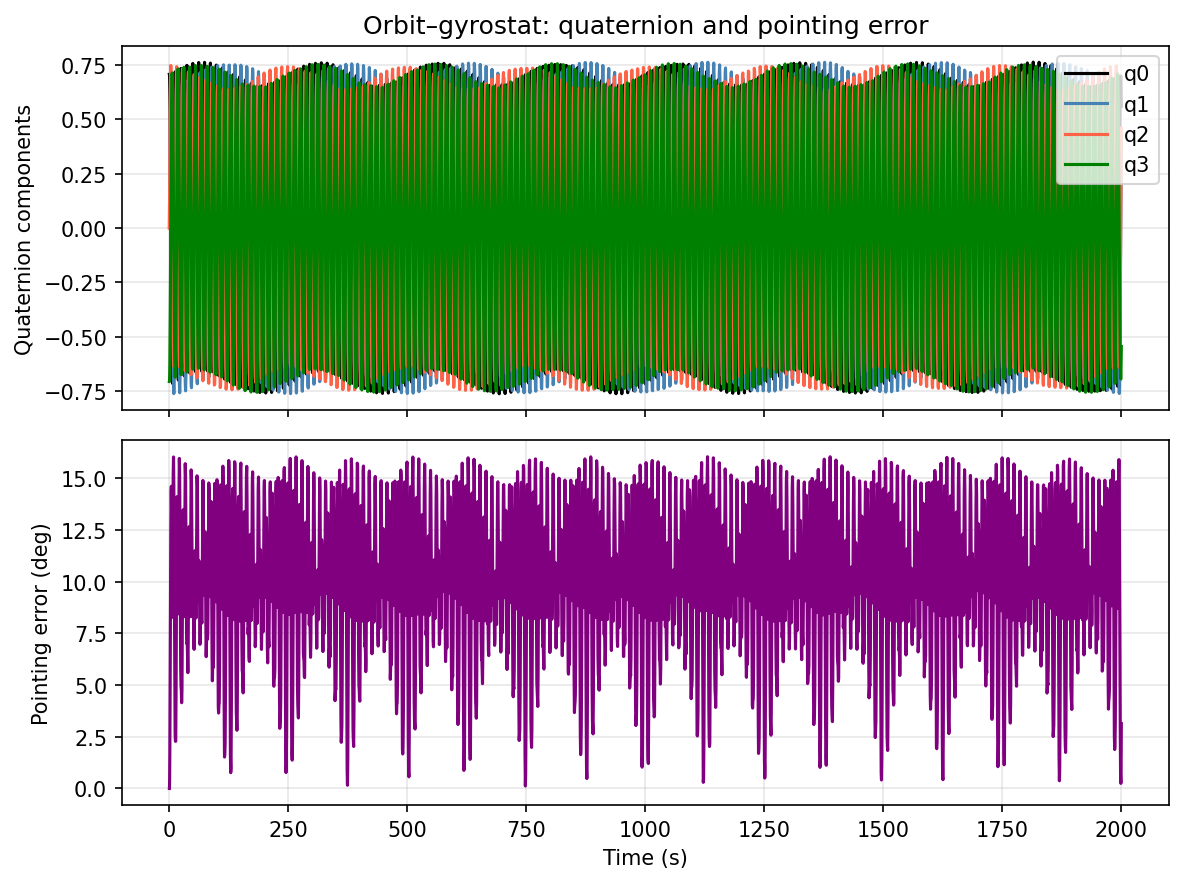
\includegraphics[width=0.78\linewidth]{figs/orbit_attitude_and_pointing.png}
    \caption{Coupled orbit-gyrostat simulation showing quaternion evolution and solar panel pointing error over several nutation periods.}
    \label{fig:orbit_gyrostat}
\end{figure}

\subsection{Discussion}

The safe-mode design developed here shows that a stable spin can be achieved even
when the desired spin axis is not a principal axis of the nominal spacecraft inertia.
By adding rotor momentum along the solar panel normal, the effective spin-axis
inertia is increased above the transverse inertias, creating the gyroscopic stiffness
needed for passive stability. The resulting stored momentum is modest for a 6U
spacecraft and is therefore compatible with a practical reaction-wheel-based
implementation.

The coupled orbit-attitude simulation further shows that the passive gyrostat design
remains well-behaved when embedded in the full spacecraft dynamics model. The
spacecraft exhibits bounded nutation, while the solar panel normal remains pointed
within a limited angular envelope about the Sun direction. In an operational flight
system, this safe mode would likely be entered through an active detumble and
reconfiguration sequence using magnetorquers and rate feedback. Nevertheless, the
results of this homework demonstrate that the passive equilibrium itself is stable
and suitable as a survivable fallback attitude state for the Starling spacecraft.

\section{Attitude Sensors}

Published information on the mission does not appear to include a complete list of exact flight sensor part numbers, so the approach taken here is to use a Starling-consistent sensor suite based on the Blue Canyon 6U bus and standard CubeSat ADCS architecture. For this report, the modeled attitude sensor suite consists of a sun sensor, a three-axis magnetometer, and a star tracker \cite{STARLING_OVERVIEW,BCT_XB1,BCT_XACT}.

\subsection{Summary of Modeled Sensors}

Based on the available public information, the attitude sensor suite used in this report is modeled as:
\begin{itemize}
    \item a sun sensor measuring the Sun direction in the body frame, with representative performance of \(<0.3^\circ\) accuracy and \(110^\circ\) field of view,
    \item a three-axis magnetometer measuring the geomagnetic field direction in the body frame, with representative performance of \(\pm 60{,}000\) nT range, \(\leq 8\) nT resolution, and \(<16\) nT rms/\(\sqrt{\text{Hz}}\) noise density,
    \item and a star tracker providing a fine attitude estimate with representative accuracy of \(6\) arcsec cross-boresight and \(40\) arcsec about-boresight.
\end{itemize}

The sun sensor and magnetometer will be used as the primary vector measurements for the static attitude estimation problem. The star tracker will also be assigned a covariance matrix and a noise model, even though it outputs attitude directly, so that its uncertainty is represented consistently within the overall sensor model.


\subsection{Sun Sensor}

The sun sensor provides a measurement of the Sun direction expressed in the spacecraft body frame. This makes it a natural sensor for  attitude knowledge, safe mode recovery, and any attitude determination problem in which the inertial Sun direction is known from ephemeris data. In this report, the sun sensor measurement is treated as a noisy unit direction vector,
\[
{}^{B}\hat{s},
\]
representing the measured Sun direction in the body frame. The AAC Clyde Space SS200 reports a field of view of \(110^\circ\), an accuracy of less than \(0.3^\circ\) (1-\(\sigma\)) over the \(\pm 45^\circ\) range, and a sampling rate up to \(10\) Hz \cite{AAC_SS200}.

\subsection{Magnetometer}

The three-axis magnetometer provides a measurement of the local geomagnetic field vector in the spacecraft body frame,
\[
{}^{B}\hat{m}.
\]

Magnetometer performance is reported in magnetic field units rather than directly as an angular error. For the representative sensor used here, the NewSpace Systems three-axis magnetometer reports a measurement range of \(\pm 60{,}000\) nT, a resolution of at most \(8\) nT, a noise density below \(16\) nT rms/\(\sqrt{\text{Hz}}\) at \(1\) Hz, and axis orthogonality error below \(1^\circ\) \cite{NSS_MAG}. These values are still useful, but they require an additional modeling step before they can be used in an attitude estimation covariance matrix. 

\subsection{Star Tracker}

The star tracker serves as the fine attitude sensor in this modeled sensor suite. Unlike the sun sensor and magnetometer, which measure individual reference directions, the star tracker estimates the spacecraft attitude directly. Blue Canyon material for nano star trackers reports attitude errors on the order of arcseconds \cite{BCT_NST}.

For the sensor used here, the Blue Canyon standard nano star tracker reports a cross-boresight accuracy of \(6\) arcsec and an about-boresight accuracy of \(40\) arcsec \cite{BCT_NST}. Even though the star tracker is not used in exactly the same way as the sun sensor and magnetometer in the Wahba formulation, it should still be included in the sensor characterization. It has finite error, and that error should still be captured with a covariance model.

\subsection{Sensor Covariance Matrices}

With the specifications established, covariance matrices can now be assigned for use in the measurement simulation. In each case, the published \(1\sigma\) accuracy is first converted to radians, then squared to obtain the corresponding variance.

\subsubsection{Sun Sensor Covariance}

For the sun sensor, a representative \(1\sigma\) angular accuracy of \(0.3^\circ\) is used. Converting to radians gives
\[
\sigma_s = 0.3\frac{\pi}{180} \approx 5.236\times 10^{-3}\ \text{rad}.
\]
The corresponding variance is
\[
\sigma_s^2 \approx 2.74\times 10^{-5}\ \text{rad}^2.
\]
The sun sensor covariance matrix is therefore modeled as
\[
R_s
=
\begin{bmatrix}
2.74\times 10^{-5} & 0 & 0 \\
0 & 2.74\times 10^{-5} & 0 \\
0 & 0 & 2.74\times 10^{-5}
\end{bmatrix}.
\]

\subsubsection{Magnetometer Covariance}

For the magnetometer, an effective \(1\sigma\) directional uncertainty of \(1.0^\circ\) is adopted for the attitude estimation model. Converting to radians gives
\[
\sigma_m = 1.0\frac{\pi}{180} \approx 1.745\times 10^{-2}\ \text{rad}.
\]
The corresponding variance is
\[
\sigma_m^2 \approx 3.05\times 10^{-4}\ \text{rad}^2.
\]
The magnetometer covariance matrix is then taken as
\[
R_m
=
\begin{bmatrix}
3.05\times 10^{-4} & 0 & 0 \\
0 & 3.05\times 10^{-4} & 0 \\
0 & 0 & 3.05\times 10^{-4}
\end{bmatrix}.
\]

\subsubsection{Star Tracker Covariance}

For the star tracker, Blue Canyon reports a cross-boresight accuracy of \(6\) arcsec and an about-boresight accuracy of \(40\) arcsec. Converting from arcseconds to radians gives
\[
\sigma_{\perp} = 6\left(\frac{1}{3600}\right)\frac{\pi}{180}
\approx 2.91\times 10^{-5}\ \text{rad},
\]
\[
\sigma_{\parallel} = 40\left(\frac{1}{3600}\right)\frac{\pi}{180}
\approx 1.94\times 10^{-4}\ \text{rad}.
\]
Squaring these values gives
\[
\sigma_{\perp}^2 \approx 8.46\times 10^{-10}\ \text{rad}^2,
\qquad
\sigma_{\parallel}^2 \approx 3.76\times 10^{-8}\ \text{rad}^2.
\]
Assuming the boresight is aligned with the third sensor axis, the star tracker covariance matrix is modeled as
\[
R_{st}
=
\begin{bmatrix}
8.46\times 10^{-10} & 0 & 0 \\
0 & 8.46\times 10^{-10} & 0 \\
0 & 0 & 3.76\times 10^{-8}
\end{bmatrix}.
\]

These covariance matrices provide the noise levels used in the sensor simulation for the remainder of this report. The sun sensor and magnetometer covariances are used directly in the vector measurement generation, while the star tracker covariance is used to model uncertainty in the fine attitude estimate.

\subsection{Simulated Measurement Generation}

With the sensor covariance matrices, simulated measurements can now be generated for use in the attitude estimation algorithms. For the sun sensor and magnetometer, the underlying quantity of interest is a unit direction vector in the spacecraft body frame. Let the true body-frame reference vector be denoted by
\[
{}^{B}v_{\text{true}} \in \mathbb{R}^3,
\qquad
\|{}^{B}v_{\text{true}}\| = 1.
\]
A noisy sensor measurement is generated by adding zero-mean Gaussian noise with covariance \(R\):
\[
n \sim \mathcal{N}(0,R),
\]
\[
{}^{B}\tilde{v} = {}^{B}v_{\text{true}} + n.
\]
Since the sun sensor and magnetometer are modeled as direction measurements, the resulting vector is then normalized so that the simulated measurement remains a unit vector:
\[
{}^{B}v_{\text{meas}}
=
\frac{{}^{B}\tilde{v}}{\|{}^{B}\tilde{v}\|}.
\]
This same measurement model is used for both the sun sensor and the magnetometer, with the only difference being the covariance matrix used to generate the noise:
\[
{}^{B}s_{\text{meas}}
=
\frac{{}^{B}s_{\text{true}} + n_s}{\|{}^{B}s_{\text{true}} + n_s\|},
\qquad
n_s \sim \mathcal{N}(0,R_s),
\]
\[
{}^{B}m_{\text{meas}}
=
\frac{{}^{B}m_{\text{true}} + n_m}{\|{}^{B}m_{\text{true}} + n_m\|},
\qquad
n_m \sim \mathcal{N}(0,R_m).
\]

The star tracker is modeled slightly differently. Rather than measuring a single reference vector, it provides an attitude estimate directly. Its noise is therefore represented as a small attitude error applied to the true attitude. Let the true spacecraft attitude be represented by a quaternion
\[
q_{\text{true}}.
\]
A small star tracker error is modeled by sampling an attitude perturbation vector
\[
\delta\phi \sim \mathcal{N}(0,R_{st}),
\]
where \(R_{st}\) is the star tracker covariance matrix defined previously. For small angles, this perturbation can be converted into an error quaternion
\[
\delta q \approx
\begin{bmatrix}
1 \\
\tfrac{1}{2}\delta\phi
\end{bmatrix},
\]
followed by normalization if needed. The measured star tracker attitude is then formed by composing the true attitude with this small perturbation:
\[
q_{\text{meas}} = q_{\text{true}} \otimes \delta q.
\]

\subsection{Monte Carlo Verification}

To verify that the simulated measurements reproduce the intended noise statistics, Monte Carlo trials were run for each sensor with $N = 10{,}000$ independent samples drawn from a fixed true reference direction or attitude.

For the sun sensor and magnetometer, the true reference vector was held fixed and $N$ noisy unit-vector measurements were generated. The angular error per sample was computed as the arc-angle between the noisy and true vectors. Because the additive Gaussian noise is isotropic in three dimensions but the result is projected onto the unit sphere, the transverse component of the noise—which drives the angular error—has two degrees of freedom. The angular error therefore follows a Rayleigh distribution with parameter $\sigma$:
\[
f(\theta;\,\sigma)
= \frac{\theta}{\sigma^2}\exp\!\left(-\frac{\theta^2}{2\sigma^2}\right),
\qquad \theta \geq 0,
\]
whose mean is $\sigma\sqrt{\pi/2}$ and whose RMS is $\sigma\sqrt{2}$. Table~\ref{tab:sec3_mc} summarizes the sample statistics against these theoretical predictions.

\begin{table}[H]
\centering
\begin{tabular}{lcccc}
\hline
\textbf{Sensor} & \textbf{Intended }$\sigma$ & \textbf{Theory mean} & \textbf{Sample mean} & \textbf{Sample RMS} \\
\hline
Sun sensor     & $0.300$° & $0.376$° & $0.379$° & $0.428$° \\
Magnetometer   & $1.000$° & $1.253$° & $1.247$° & $1.409$° \\
\hline
\end{tabular}
\caption{Monte Carlo angular error statistics for vector sensors ($N=10{,}000$). Theory and sample values agree to within 1\%, confirming correct noise generation.}
\label{tab:sec3_mc}
\end{table}

For the star tracker, the identity attitude was used as the true reference and $N$ noisy quaternion measurements were generated. The perturbation vector $\delta\phi$ was recovered from each measurement as $\delta\hat{\phi} = 2\,\mathrm{logq}(q_{\text{meas}})$, and the sample covariance of these vectors was compared to $R_{st}$. The recovered per-axis standard deviations were $5.91$ arcsec, $6.00$ arcsec, and $40.24$ arcsec against intended values of $6$, $6$, and $40$ arcsec, confirming the anisotropic noise model is correctly implemented.

Figure~\ref{fig:sensor_verification} shows the angular error histograms for the sun sensor and magnetometer overlaid with the theoretical Rayleigh distributions, and the per-axis perturbation histograms for the star tracker.

\begin{figure}[H]
    \centering
    
\includegraphics[width=\linewidth]{figs/sensor_noise_verification.png}
    \caption{Monte Carlo verification of sensor noise models ($N = 10{,}000$ trials). \textit{Left, center}: angular error histograms for the sun sensor (0.3° 1$\sigma$) and magnetometer (1.0° 1$\sigma$) overlaid with the theoretical Rayleigh distribution. \textit{Right}: per-axis attitude perturbation histograms for the star tracker, showing the asymmetry between the 6 arcsec cross-boresight axes and the 40 arcsec about-boresight axis.}
    \label{fig:sensor_verification}
\end{figure}

\section{Static Attitude Estimation (Wahba's Problem)}

\subsection{Problem Formulation}

Using the noisy sensor models from Section~3, we perform static attitude estimation by solving Wahba's problem \cite{Wahba1965}: given unit-vector measurements ${}^B b_k$ in the body frame and corresponding inertial reference vectors ${}^N r_k$, find the rotation matrix $A$ minimizing the weighted sum of squared residuals,
\[
\min_{A \in SO(3)}
\sum_{k=1}^{n} w_k \,\bigl\| {}^B b_k - A\, {}^N r_k \bigr\|^2,
\]
where $w_k > 0$ are weights reflecting each sensor's accuracy.

\subsection{Sensor Selection for Wahba's Problem}

The sun sensor and magnetometer each produce a body-frame unit-vector measurement that can be paired with a known inertial reference—the Sun direction from ephemeris and the geomagnetic field from a magnetic model, respectively—making both natural inputs to Wahba's problem.

The star tracker computes a full three-axis attitude quaternion internally and its output is not a body/inertial vector pair, so it cannot enter the Wahba formulation directly here. Its role in the sensor architecture is as a standalone fine-attitude source when available.

\subsection{Reference Geometry and Weights}

The inertial Sun direction was taken as the ECI $+x$ axis (consistent with Section~2) and the magnetic reference as ${}^N r_m = \mathrm{normalize}([0.3,\,0.5,\,0.8]^T)$. The two vectors are separated by $72°$ (dot product $0.303$), well away from the degenerate parallel case that would leave the spin-axis degree of freedom unobservable.

Sensor weights were set proportional to inverse variance and normalized to unity:
\[
w_s = \frac{1/\sigma_s^2}{1/\sigma_s^2 + 1/\sigma_m^2} \approx 0.917,
\qquad
w_m = \frac{1/\sigma_m^2}{1/\sigma_s^2 + 1/\sigma_m^2} \approx 0.083,
\]
giving the sun sensor approximately eleven times the weight of the magnetometer.

\subsection{Algorithm 1: SVD Method}

The SVD solution \cite{Markley1988} forms the attitude profile matrix
\[
B = \sum_{k=1}^{n} w_k\, {}^B b_k\, ({}^N r_k)^T,
\]
computes its SVD $B = U\Sigma V^T$, and recovers the optimal rotation as
\[
A_{\text{SVD}}
= V \,\mathrm{diag}\!\left(1,\,1,\,\det(V)\det(U)\right) U^T,
\]
where the diagonal correction enforces $\det(A_{\text{SVD}}) = +1$.

\subsection{Algorithm 2: Davenport q-Method}

The Davenport q-method \cite{Davenport1968} works directly in quaternion space. The $4 \times 4$ Davenport matrix is assembled as
\[
D = \sum_{k=1}^{n} w_k\, L(H\, {}^N r_k)^T R(H\, {}^B b_k),
\]
where $L(\cdot)$ and $R(\cdot)$ are quaternion left- and right-multiplication matrices and $H = [0_{1\times3};\; I_3]$ embeds a three-vector as a pure quaternion. The optimal quaternion is the eigenvector of $D$ at its maximum eigenvalue.

\subsection{Monte Carlo Comparison}

Both algorithms were evaluated over $N = 5{,}000$ Monte Carlo trials with randomly generated true attitudes and noisy sun and magnetometer measurements drawn from the Section~3 models. The attitude error per trial is the three-dimensional rotation angle
\[
\theta_{\text{err}}
= \frac{180}{\pi}\,\bigl\|\,\mathrm{unhat}\!\bigl(\log(A_{\text{est}}^T A_{\text{true}})\bigr)\bigr\|.
\]

Results are summarized in Table~\ref{tab:wahba_mc} and shown in Figure~\ref{fig:wahba_comparison}.

\begin{table}[H]
\centering
\begin{tabular}{lccccr}
\hline
\textbf{Algorithm} & \textbf{Mean} & \textbf{Std} & \textbf{RMS} & \textbf{95th pctile} & \textbf{Time (5000 trials)} \\
\hline
SVD            & $0.971$° & $0.578$° & $1.130$° & $2.093$° & $0.036$ s \\
Davenport q    & $0.975$° & $0.582$° & $1.135$° & $2.109$° & $0.179$ s \\
\hline
\end{tabular}
\caption{Monte Carlo attitude estimation accuracy and computational cost ($N = 5{,}000$ trials). Both methods solve the same optimization problem and produce statistically identical results. The SVD method is approximately five times faster.}
\label{tab:wahba_mc}
\end{table}

\begin{figure}[H]
    \centering
    
\includegraphics[width=\linewidth]{figs/wahba_comparison.png}
    \caption{Monte Carlo comparison of SVD and Davenport q-method attitude estimation ($N = 5{,}000$ trials). \textit{Left}: overlaid error histograms showing the right-skewed distribution characteristic of a 3D rotation error with anisotropic sensor noise. \textit{Right}: empirical CDFs; the two curves overlap, confirming equivalent accuracy.}
    \label{fig:wahba_comparison}
\end{figure}

\subsection{Discussion}

Both algorithms are exact solvers for the same problem and produce statistically indistinguishable results. The SVD method is approximately five times faster, as it requires a $3\times3$ decomposition rather than a $4\times4$ eigendecomposition.

The $\sim$1° mean error is consistent with what the two-vector geometry predicts. The sun sensor constrains the two degrees of freedom transverse to the Sun direction at $\sigma_s = 0.3°$; the remaining degree of freedom (rotation about the Sun vector) is constrained only by the magnetometer, whose effective accuracy along that axis is $\sigma_m / \sin\theta_{sm} \approx 1.0° / \sin(72°) \approx 1.05°$. The expected RMS is therefore
\[
\text{RMS} \approx \sqrt{2\sigma_s^2 + (\sigma_m/\sin\theta_{sm})^2}
= \sqrt{2(0.3°)^2 + (1.05°)^2}
\approx 1.13°,
\]
in close agreement with the simulated value of $1.130°$. The magnetometer is the dominant error source; The star tracker, when available, reduces this limitation by providing direct attitude measurements with arcsecond-level accuracy.

\newpage

\begin{thebibliography}{99}

\bibitem{Wahba1965}
G.~Wahba,
``A Least Squares Estimate of Spacecraft Attitude,''
\textit{SIAM Review}, vol.~7, no.~3, p.~409, 1965.

\bibitem{Markley1988}
F.~L. Markley,
``Attitude Determination Using Vector Observations and the Singular Value Decomposition,''
\textit{Journal of the Astronautical Sciences}, vol.~36, no.~3, pp.~245--258, 1988.

\bibitem{Davenport1968}
P.~B. Davenport,
``A Vector Approach to the Algebra of Rotations with Applications,''
NASA Technical Note TN D-4696, 1968.

\bibitem{SMAD}
Wertz, J. R., and Larson, W. J.,
\textit{Space Mission Analysis and Design (SMAD)},
Microcosm Press.

\bibitem{STARLING_OVERVIEW}
NASA,
``Starling Mission Overview,''
NASA Mission Page,
\url{https://www.nasa.gov/mission/starling/}

\bibitem{STARLING_FLIGHT}
Miller, S. et al.,
``Starling CubeSat Swarm Technology Demonstration Flight Results,''
NASA Technical Reports Server (NTRS), 2024,
\url{https://ntrs.nasa.gov/}

\bibitem{BCT_XB1}
Blue Canyon Technologies,
``XB1 6U CubeSat Bus Overview,''
Product Documentation,
\url{https://www.bluecanyontech.com/spacecraft/6u-cubesat/}

\bibitem{BCT_XACT}
Blue Canyon Technologies,
``XACT Attitude Determination and Control System,''
Product Documentation,
\url{https://www.bluecanyontech.com/spacecraft-subsystems/xact/}

\bibitem{Vallado2013}
D.~A. Vallado,
\textit{Fundamentals of Astrodynamics and Applications}, 4th~ed.,
Microcosm Press / Springer, 2013.

\bibitem{Curtis2014}
H.~D. Curtis,
\textit{Orbital Mechanics for Engineering Students}, 3rd~ed.,
Butterworth-Heinemann / Elsevier, 2014.

\bibitem{EGM96}
F.~G. Lemoine et al.,
``Development of the Joint NASA GSFC and NIMA Geopotential Model EGM96,''
NASA/TP-1998-206861, NASA Goddard Space Flight Center, 1998.

\bibitem{NASA_GNC}
NASA,
``State of the Art of Small Spacecraft Technology: Guidance, Navigation, and Control,''
NASA Small Spacecraft Systems Virtual Institute,
\url{https://www.nasa.gov/smallsat-institute/sst-soa/guidance-navigation-and-control/}

\bibitem{AAC_SS200}
AAC Clyde Space,
``SS200 Digital Sun Sensor,''
Product Documentation.

\bibitem{NSS_MAG}
NewSpace Systems,
``Space Magnetometer Datasheet,''
Product Documentation.

\bibitem{BCT_NST}
Blue Canyon Technologies,
``Nano Star Tracker,''
Product Documentation,
\url{https://www.bluecanyontech.com/components/nano-star-trackers/}

\end{thebibliography}

\end{document}